\documentclass[11pt,a4paper]{article}
\usepackage{authblk}
\usepackage{amsmath}
\usepackage{booktabs}
%\usepackage{ctex}
\usepackage{caption}  
\usepackage{changepage}
\usepackage{diagbox}
\usepackage{float}
\usepackage[T1]{fontenc}
\usepackage{geometry}
\usepackage[utf8]{inputenc}
 \usepackage{pgfplots}
 \usepgfplotslibrary{dateplot}
\usepackage{multicol}
\usepackage{multirow}
\usepackage{listings}
\usepackage{subfigure}
\usepackage{tcolorbox}
\usepackage{threeparttable}
\usepackage{xpinyin}
\usepackage{xcolor}
\usepackage{listings}
\usepackage{fontspec}
\usepackage{hyperref}

\definecolor{commentColor}{RGB}{53,129,34}
\definecolor{keywordColor}{RGB}{199, 117, 50}
\definecolor{stringColor}{RGB}{98, 123, 83}
\definecolor{preprocessorColor}{RGB}{114, 75, 48}
\definecolor{characterColor}{RGB}{31, 53, 207}
\definecolor{numberColor}{RGB}{166, 166, 166}
\definecolor{oglobalColor}{RGB}{97, 64, 154}
\definecolor{globalColor}{RGB}{89, 127, 134}
\definecolor{functionColor}{RGB}{135,135,197}
\definecolor{classColor}{RGB}{146,84,139}

\lstset{language=python,
keywordstyle=\color{keywordColor},
commentstyle=\color{commentColor},
stringstyle=\color{stringColor},
showstringspaces=false,
columns=fullflexible,keepspaces,
numbers=left,
numberstyle=\color{numberColor}\footnotesize,
keywords=[2]{std, cout, cin},
keywordstyle = [2]{\color{oglobalColor}},
keywords=[3]{endl, print, scanf, setw, setfill, setbase, setprecision, time, ctime, rand, len},
keywordstyle = [3]{\color{functionColor}},
keywords=[4]{\#include},
keywordstyle =[4]{\color{preprocessorColor}},
keywords=[5]{self},
keywordstyle =[5]{\color{classColor}},
literate={
    {<<}{{{\color{black}<<}}}1
    {>>}{{{\color{black}>>}}}1
    {*}{{{*}}}1
    {0}{{{\color{characterColor}0}}}1
    {1}{{{\color{characterColor}1}}}1
    {2}{{{\color{characterColor}2}}}1
    {3}{{{\color{characterColor}3}}}1
    {4}{{{\color{characterColor}4}}}1
    {5}{{{\color{characterColor}5}}}1
    {6}{{{\color{characterColor}6}}}1
    {7}{{{\color{characterColor}7}}}1
    {8}{{{\color{characterColor}8}}}1
    {9}{{{\color{characterColor}9}}}1},
tabsize=4
}

\geometry{top=1.5cm,bottom=1.5cm,left=1.5cm,right=1.5cm}

\title{Math 286 Lab Project}
\date{2020, Sept, 11th}
\author{\textbf{Ruan Yucheng} 3180111636}
\author{\textbf{Zhang Zheyuan} 3180111607}
\author{\textbf{Wu Zheyu} 3180111600}
\author{\textbf{Qian Chen} 3180111591}
\author{\textbf{Zheng Xiuwen} 3180111639}
\affil{We declare that this report is our own original work, and every work group member has a fair share in this work. For the preparation of the report we have not used any other resources than the Math 286 lecture material and the references cited in the report.}
\renewcommand\Authands{ and }

\setlength{\textfloatsep}{5pt}

\hypersetup{
	colorlinks=true,
	linkcolor=black
}

\begin{document}
\setlength{\parindent}{0pt}
\maketitle

\section{Problem 1}
Determine the maximal solution of the following ODE with the initial value.
\begin{equation}
	y' = t^2+y^3, y(0)=1	\tag{IVP1}  \label{IVP1}
\end{equation}
\subsection{Direction Field}
At first, we plot the direction field of (1). After connecting the direction arrows we find that the curve seems has 2 vertical asymptotes, which approximately lies between -2.1 to -2.2 and 0.8 to 0.9.

\begin{center}
	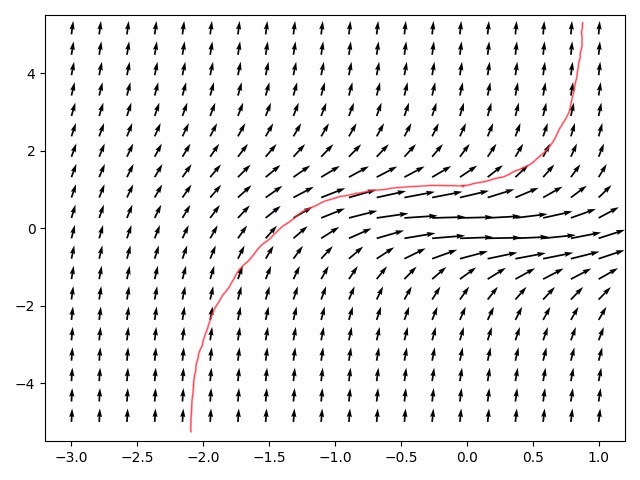
\includegraphics[scale=0.2]{HandSketch.jpeg}
\end{center}

\subsection{Numerical Methods}

\subsubsection{Methods}
\begin{table}[H]
	\begin{center}
		\scriptsize
		\renewcommand{\arraystretch}{1.3} % default is 1.0
		\begin{tabular}{p{8cm}|p{8cm}}
			\textbf{Euler}: \hyperref[Euler]{<code>}		& \quad\textbf{Heun}: \hyperref[Heun]{<code>}				\\
			$y_{n+1} = y_n+h \cdot f(t_n, y_n)$	& \quad$ k_{1,n} = f(t_n,y_n)$				\\
			$ t_{n+1} = t_n+h$				& \quad$ k_{2,n} = f(t_n+h, y_n+h \cdot k_{1,n})$	\\
											& \quad$ y_{n+1} = y_n+h \cdot f(t_n, y_n)$		\\
											& \quad$ t_{n+1} = t_n+h$					\\
										 	
			
			\textbf{Runge Kutta}: \hyperref[Runge Kutta]{<code>}										&					\\
			$ k_{1,n} = f(t_n,y_n)$												&					\\
			$ k_{2,n} = f(t_n+\frac{h}{2}, y_n+\frac{h}{2} \cdot k_{1,n})$			&					\\
			$ k_{3,n} = f(t_n+\frac{h}{2}, y_n+\frac{h}{2} \cdot k_{2,n})$			&					\\
			$ k_{4,n} = f(t_n+h, y_n+h \cdot k_{3,n})$								&					\\
			$ y_{n+1} = y_n+\frac{h}{6} \cdot (k_{1,n}+2 \cdot (k_{2,n}+k_{3,n})+k_{4,n})$	&					\\
			$ t_{n+1} = t_n+h$													&					\\
		\end{tabular}
	\end{center}
\end{table}

\subsubsection{Approximation}
We apply three methods all together with a step of $h = 0.1$ obtain the table below:
\begin{table}[H]
	\begin{center}
		\scriptsize
		\renewcommand{\arraystretch}{1.2} % default is 1.0
		\begin{tabular}{l|r|r|r|r|r|r|r|r}
			\textbf{T}	&\textbf{-2.3}	&\textbf{-2.2}	&\textbf{-2.1}	&\textbf{-2.0}	&\textbf{0.7}	&\textbf{0.8}	&\textbf{0.9}	&\textbf{1.0}	\\
			\hline
			Euler		&-19.87			&-9.10			&-5.05			&-3.08			&3.41			&4.85			&7.66			&14.31			\\	
			\hline
			Heun		&-5.48E5		&-175.74		&-17.44			&-6.25			&5.36			&11.14			&48.95			&4479.18		\\
			\hline
			RK			&-1.62E99		&-2.59E7		&-36.57			&-7.12			&5.89			&16.04			&2777.84		&5.43E35		\\
		\end{tabular}
	\end{center}
\end{table}

Combined with the table, the direction field and the hand-drawing sketches, we could find that the results diverses dramatically large around -2.2 to -2.1 and 0.8 to 0.9. Which may conform with our initial observation. To verify this we apply three methods altogether with smaller steps at these points.

\begin{table}[H]
	\scriptsize
	
	\begin{center}
		\begin{threeparttable}
			\renewcommand{\arraystretch}{1.2} % default is 1.0
			\begin{tabular}{r|r|r|r|r|r|r|r|r|r|r|r|r}
				\multirow{2}*{\diagbox{h}{t}}&\multicolumn{3}{c|}{-2.2} &\multicolumn{3}{c|}{-2.1}&\multicolumn{3}{c|}{0.8}&\multicolumn{3}{c}{0.9} \\
				\cline{2-13}
						&Euler	&Heun			&RK		&Euler	&Heun	&RK		&Euler	&Heun	&RK		&Euler	&Heun	&RK		\\
				\hline
				0.05 	&-12.20	&-151.20		&-1.22E5&-5.61	&-11.55	&-13.01	&5.16	&8.23	&8.77	&9.27	&34.28	&81.49	\\
				0.01 	&-1.43E5&-inf\tnote{*}	&-inf	&-16.81	&-30.33	&-31.53	&10.67	&13.98	&14.10	&103.56	&5.96E26&inf	\\
				0.001	&-inf	&-inf			&-inf	&-38.88	&-45.05	&-45.09	&15.60	&16.28	&16.28	&inf	&inf	&inf	\\
				0.0001	&-inf	&-inf			&-inf	&-46.29	&-47.10	&-47.10	&16.46	&16.54	&16.55	&inf	&inf	&inf
			\end{tabular}
			\begin{tablenotes}
				\footnotesize
				\item[*] inf stands that the calculated result is larger than the largest number that can be hold by numpy.
			\end{tablenotes}
			\setlength{\abovecaptionskip}{0.1cm}
			\setlength{\belowcaptionskip}{-0.9cm}
			\caption{Calculated Results in Different $h$}\label{tab:tab1.2.2.1}
		\end{threeparttable}
		
	\end{center}
\end{table}
From Table \ref{tab:tab1.2.2.1} we could find that $y$ at $t = -2.2$ and $t = 0.9$ if we decrease the step size, the value will increase/decrease rapidly and finally exceed the range that numpy can hold. But when $t = -2.1$ and $t = 0.8$, $y$ will finally get to a certain value.

The large difference among the computed values with different step sizes at $t = -2.2$ and $t = 0.9$ indicated that there may has 2 vertical asymptotes lies in $-2.2<t<2.1$ and $0.8<t<0.9$, respectively. To narrow down the interval, we chose fourth order  Runge-Kutta method with a smaller step size $h=0.0000001$. In comparision, we also compute the Improved Euler (Heun) Method's results.

\begin{table}[H]
	\scriptsize
	
	\begin{center}
		\renewcommand{\arraystretch}{1.2} % default is 1.0
		\begin{tabular}{l|r|r|r|r|r|r|r}
			\textbf{T}	&\textbf{-2.1206582}	&\textbf{-2.1206583}	&\textbf{-2.1206584}	&\textbf{-2.1206585}		&\textbf{-2.1206586}	&\textbf{-2.1206587}	&\textbf{-2.1206588}	\\
			\hline
			Heun		&-3354392.36			&-4920325.98			&-8825532.00			&-26522181.22				&-530832939.07			&-4.12E+33				&-1.44E+33				\\
			\hline
			RK			&-3520929.53			&-5430876.24			&-11766978.25			&-211743592.76				&-1.37E+24				&-6.39E+276				&-inf					\\
		\end{tabular}
		\setlength{\abovecaptionskip}{0.1cm}
		\setlength{\belowcaptionskip}{-0.9cm}
		\caption{Runge Kutta and Heun Results with $h=0.0000001$ around -2.1}\label{tab:tab1.2.2.2}
	\end{center}
	
\end{table}

\begin{table}[H]
	\scriptsize
	
	\begin{center}
		\renewcommand{\arraystretch}{1.2} % default is 1.0
		\begin{tabular}{l|r|r|r|r|r|r}
			\textbf{T}	&\textbf{0.8588757}	&\textbf{0.8588758}	&\textbf{0.8588759}	&\textbf{0.8588760}		&\textbf{0.8588761}	&\textbf{0.8588762}	\\
			\hline
			Heun		&3478801.43			&5183244.40			&9623270.74			&32083922.20			&995096229.24		&500217988540590.00	\\
			\hline
			RK			&3664014.20			&5778202.21			&13477433.90		&537639394.88			&2.66E+30			&inf				\\
		\end{tabular}
		\setlength{\abovecaptionskip}{0.1cm}
		\setlength{\belowcaptionskip}{-0.9cm}
		\caption{Runge Kutta and Heun Results with $h=0.0000001$ around 0.8}\label{tab:tab1.2.2.3}
	\end{center}
	
\end{table}
From Table \ref{tab:tab1.2.2.2} and Table \ref{tab:tab1.2.2.3} we could find there two abrupt increments, which are located at around -2.1206585 to -2.1206586 and 0.8588759 to 0.8588761, respectively. Based on this we could obtain two asymptotes with 6 digit accuracy, which are -2.120659 and 0.858876. In other words, the domain of \ref{IVP1} is $(-2.120659, 0.858876)$.

\subsection{Analytical Methods}
\subsubsection{Power Series}
\begin{table}[H]
	\scriptsize
	\begin{center}
		\renewcommand{\arraystretch}{2} % default is 1.0
		\begin{tabular}{p{10cm}|p{10cm}}
			$y = \sum_{n=0}^{\infty}a_n \cdot t^n$									&\quad$n=0, a_1=a_0^2$\\
			$y'= \sum_{n=0}^{\infty}a_{n+1} \cdot t^n$								&\quad$n=1, 2 \cdot a_2=2 \cdot a_0 \cdot a_1+a_0$\\
			$t \cdot y = \sum_{n=0}^{\infty}a_n \cdot t^{n+1}$								&\quad$n=2, 3 \cdot a_3=1+a_1^2+2 \cdot a_0 \cdot a_2$\\
			$t^2=\sum_{n=0}^{\infty}(\sum_{k=0}^{\infty} \cdot a_k \cdot a_{n-k}) \cdot t^n$		&\quad$n\geq3, (n+1) \cdot a_{n+1}=\sum_{k=0}^{n} \cdot a_k \cdot a_{n-k}+a_{n-1}$\\
			$t^2+y^2+t \cdot y=t^2+\sum_{n=0}^{\infty}(\sum_{k=0}^{\infty} \cdot a_k \cdot a_{n-k}) \cdot t^n+\sum_{n=0}^{\infty} \cdot a_n \cdot t^{n+1}$
		\end{tabular}
	\end{center}
\end{table}

As we know $y(0)=1$, applying $a_0=1$ to the recursion formula we could obtain a equation that can be easily to calculate:
\begin{center}
	$y=1+x+1.5 \cdot x^2+2 \cdot x^3+2.125 \cdot x^4+2.5 \cdot x^5+2.8958 \cdot x^6+...$
\end{center}

In our code we could modify the number of terms based on the accuracy we need. <code>

\subsubsection{Analytical Method for Vertical Asymptotes}

	%%%%%%%%%%%%%%%%%%%%%%%%%%Right%%%%%%%%%%%%%%%%%%%%%%%%%%%%%%%%%
	\paragraph{Analytical Method on the Right.} Note that, on $0\leq t \leq 1$,

	\begin{center}
		$y'=y^2+t \cdot y+t^2 \geq t \cdot y$

		therefore $y \geq e^{\frac{t^2}{2}}>0$
	\end{center}

	Note that we have ensure that the vertical asymptote locates in the interval $0.8\leq t \leq 0.9$ from the direction field. Based on this, we could have a further squeeze formula: 
	\begin{center}
		$y^2+0.8 \cdot y+0.8^2 \leq y' = y^2+t \cdot y+t^2 \leq y^2+0.9 \cdot y+0.9^2$
	\end{center}
	Therefore, we could get the lower bound and upper bound of vertical asymptote. Considering $y_1'=y_1^2+0.9 \cdot y_1+0.9^2$ first:

	We are able to obtain th solution:
	\begin{center}
		$y_1=0.45 \cdot (\sqrt3tan(0.45 \cdot (100 \cdot sqrt3 \cdot C_1+\sqrt{3} \cdot t))-1)$
	\end{center}
	Instead of using the initial value $y(0)=1$, we use $y(0.8)=16.56526818$ which is obtained by power series to get a more accurate approximation of the vertical asymptote. Then we obtain: 
	\begin{center}
		$C_1=0.0115662936$.
	\end{center}
	We are interested in the points when $y_1 \rightarrow \infty$:
	\begin{center}
		Let $0.45 \cdot (100 \cdot \sqrt3 \cdot C_1+\sqrt3 \cdot t)=\frac{\pi}{2}, \Rightarrow t_1 = 0.85873$
	\end{center}

	We could calculate in the same method on $y_2^2+0.8 \cdot y_2+0.8^2$ and obtained the solution:

	\begin{center}
		$y_2=0.4 \cdot (\sqrt{3} \cdot tan(0.4 \cdot (24 \cdot \sqrt{3} \cdot C_2+\sqrt{3} \cdot t))-1)$
	\end{center}

	Apply the initial value $y(0.8) = 16.56526818$, we get 

	\begin{center}
		$C_2=0.056333519$
	\end{center}

	When $y_2 \rightarrow \infty$, we finally get $t_2=0.85891$

	Therefore, we conclude that the vertical asymptote on the right is within the interval:
	\begin{center}
		$0.85873 \leq t \leq 0.85891$,
	\end{center}
	 Which agrees with our results in numerical method well.
	
	%%%%%%%%%%%%%%%%%%%%%%%%%%Left%%%%%%%%%%%%%%%%%%%%%%%%%%%%%%%%%
	\paragraph{Analytical Method on the Left.} Note that, on $t \leq 0$,

	\begin{center}
		$y'=y^2+t \cdot y+t^2 \geq t \cdot y$

		therefore $y \leq -e^{-\frac{t^2}{2}} \leq 0$
	\end{center}
	Which indicates that $y' > 0$ when $t \leq 0$, so we could conclude that $y$ behaves monotonic increasing when $t \leq 0$. Therefore $y < 0$ when $t \leq 0$.

	Note that we have ensure that the vertical asymptote locates in the interval $-2.5 \leq t \leq -2$ from the direction field. Consider function $\varphi(t,y) = t \cdot y+t^2$, seeing $y$ as a constant coefficient. The axi of symmetry of the function locate $t=-\frac{y}{2}$, seeing $y$ as a constant coefficient. The axis of symmetry of the function locate $t= - \frac{y}{2}$, remembering $y<0$ when $t \leq 0$

	Based on this, we could have a further squeeze formula when $-2.5 \leq t \leq -2$

	\begin{center}
		$y^2-2 \cdot y+(-2)^2 \leq y' = y^2 + t \cdot y + t^2 \leq y^2 - 2.5 \cdot y + (-2.5)^2$
	\end{center}

	Therefore, we could get the lower bound and upper bound of vertical asymptote.

	Considering $y_1'=y_1^2-2 \cdot y_1+(-2)^2$ first:

	We are able to obtain the solution: 
	
	\begin{center}
		$y_1=\sqrt{3}tan({\sqrt{3} \cdot C_1+\sqrt{3} \cdot t})+1$
	\end{center}

	Instead of using the initial value $y(0)=1$ , we use $y(-2)=-7.1421908$ which is obtained by Runge-kutta to get a more accurate approximation of the vertical asymptote. Then we obtain: 
	
	\begin{center}
		$C_1=1.214113538$
	\end{center}

	We are interested in the points when $y_1 \rightarrow -\infty$:

	\begin{center}
		Let $\sqrt{3} \cdot C_1+\sqrt{3} \cdot t=\frac{\pi}{2}, \Rightarrow t_1 = 2.1210$
	\end{center}

	We could calculate in the same method on $y_2' = y_2 ^ 2-2.5 \cdot y_2+(-2.5)^2$ and obtain the solution:

	\begin{center}
		$y_2=\frac{5}{4} \cdot (\sqrt{3} \cdot tan(\frac{5}{4} \cdot (4 \cdot \sqrt{3} \cdot C_2+\sqrt{3} \cdot t))+1)$
	\end{center}

	 Apply the initial value $y(-2) = -7.1421908$, we get 
	\begin{center}
		$C_2 = 0.3477739645$
	\end{center}

	When $y_2 \rightarrow -\infty$, we finally get $t_2=-2.1166$

	Therefore, we conclude that the vertical asymptote on the right is within the interval:

	\begin{center}
		$-2.1210 \leq t \leq -2.1166$
	\end{center}

	Which conforms our result in numerical approximation well.

\subsection{Conclusion}

\subsubsection{Error Comparison}
 
\indent We treat the value calculated by power series at t = 0.8 (within 4000 terms) as the 'exact value'. Based on this we started our error analysis. Table \ref{tab:tab1.4.1.1} shows the values calculated by three numerical methods at t=0.8 and their error compared with the 'exact value'.We could find that in this problem, if we take the same step size, Runge-Kutta method and Improved Euler method performs better in terms of accuracy.
\begin{table}[H]
	\begin{center}
		\small
		\begin{tabular}{r|r|r|r|r|r|r}
			\renewcommand{\multirowsetup}{\centering}
			exact value:&\multirow{2}*{ Euler}&\multirow{2}*{ Euler Error}&\multirow{2}*{ Heun}&\multirow{2}*{ Heun Error}&\multirow{2}*{ Runge-Kutta}&\multirow{2}*{ RK Error}\\
			 16.565268184&&&&&&\\
			 \hline
			h = 0.01		&10.67203515	&-35.5758\%		&13.9787667		&-15.6140\%	&14.10105738	&-14.8758\%	\\
			h = 0.001		&15.60414001	&-5.8021\%		&16.27971628	&-1.7238\%	&16.28178618	&-1.7113\%	\\
			h = 0.0001		&16.46233358	&-0.6214\%		&16.53646519	&-0.1739\%	&16.53648707	&-0.1737\%	\\
			h = 0.00001		&16.55490058	&-0.0626\%		&16.56238545	&-0.0174\%	&16.56238567	&-0.0174\%	\\
			h = 0.000001	&16.56451894	&-0.0045\%		&16.56526818	&0.0000\%	&16.56526818	&0.0000\%	\\
			h = 0.0000001	&16.56519326	&-0.0005\%		&16.56526818	&0.0000\%	&16.56526818	&0.0000\%	\\
		\end{tabular}
		\setlength{\abovecaptionskip}{0.1cm}
		\setlength{\belowcaptionskip}{-0.9cm}
		\caption{Error Analysis} \label{tab:tab1.4.1.1}
	\end{center}
\end{table}

\subsubsection{Conclusion}

In this problem we try to solve the IVP $y'=y^2+t \cdot y+t^2, y(0)=1$ with three numerical method: Euler Method, Heun Method and Runge-Kutta Method. In the last section we calculated the error at $t = 0.8$ of three methods with different steps and we could find that, Runge-Kutta achieves highest accuracy under same step size. In this problem The Heun method also achieves good accuracy. But the accuracy comes with price. While calculating we found that Euler Method is faster than the other two methods. The gap is widened when smaller step was applied. We recorded the time each method spent under the condition that $h=0.0000001$ and found that the Heun Method spent about 1 time longer than Euler, while Runge-Kutta roughly spent 3 times longer.

\begin{table}[H]
	\begin{center}
		\small
		\begin{tabular}{c|c|c}
			\renewcommand{\multirowsetup}{\centering}
			Euler			&Heun			&Runge Kutta	\\ \hline
			8.82 sec		&18.71 sec		&41.04 sec		\\
		\end{tabular}
		\setlength{\abovecaptionskip}{0.1cm}
		\setlength{\belowcaptionskip}{-0.9cm}
		\caption{Time Spent to Calculate $y(0.8), h = 0.0000001$} \label{tab:tab1.4.2.1}
	\end{center}
\end{table}

During our calculation, we find that the values closed to the asymptotes are more than tricky. Therefore, to determine the more accurate locations of asymptotes and verify our numerical methods, squeeze rule has been used. Figure \ref{fig:1.4.2.1} is the plot based on Runge-Kutta method with step size 0.0000001.

\begin{center}
	\begin{figure}[H]
		\centering
		\begin{minipage}[b]{0.4\textwidth}
			\centering
			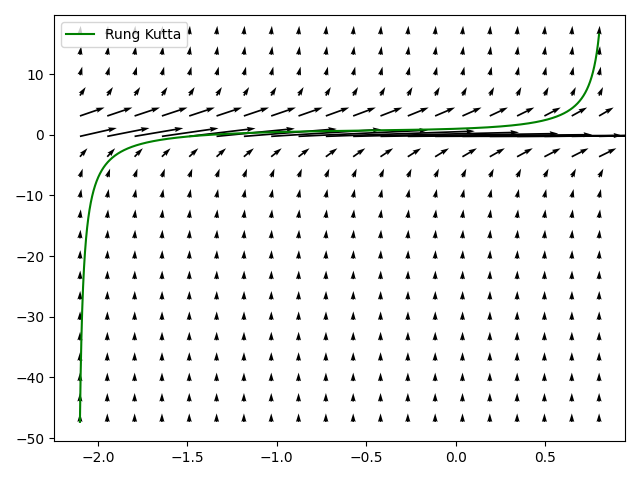
\includegraphics[width=0.7\textwidth]{P1FinalSolution.png}
			\caption{RK with h=0.0000001}
			\label{fig:1.4.2.1}
		\end{minipage}
		\begin{minipage}[b]{0.4\textwidth}
			\centering
			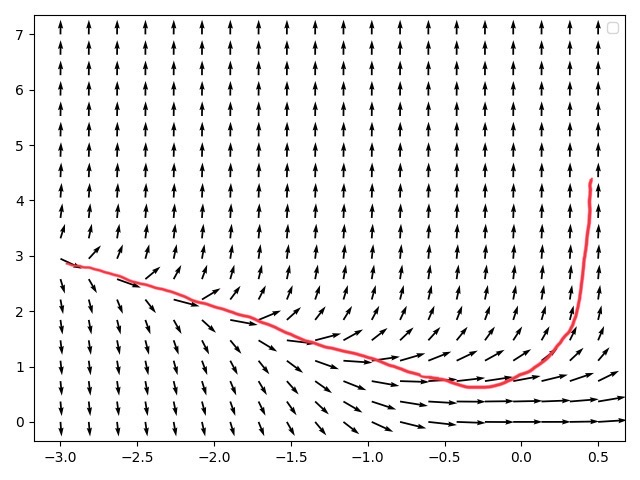
\includegraphics[width=0.7\textwidth]{Problem2HandSketch.jpeg}
			\caption{Hand-drawn Curve of Problem2}
			\label{fig:2.0.1}
		\end{minipage}

	\end{figure}
\end{center}

\section{Problem2}

Determine the maximal solution of the following ODE with the initial value.

\begin{equation}
	y' = y^3+t \cdot y^3 + t^2 \cdot y + t^3, y(0)=1 \tag{IVP2} \label{IVP2}
\end{equation}

\subsection{Direction Field}

First First, we draw the direction field of \ref{IVP2}. We can infer from the figure that the solution to problem 2 with initial value $y(0) = 1$ has a right vertical asymptote between 0.4 and 0.5. Besides, it seems that the solution has a left slanted asymptote.

\subsection{Numerical Analysis}

We use Runge-Kutta Method with step $h=0.01$ to checkout that the graph we draw is roughly right.

\begin{table}[H]
	\centering
	\begin{tabular}{l|l|l|l|l|l|l|l}
		step h & t=-10 & t=-5  & t=-1  & t=-0.5 & t=0 & t=0.2 & t=0.4 \\
		\hline
		0.01   & 9.985 & 4.970 & 0.771 & 0.756  & 1   & 1.307 & 3.019
	\end{tabular}
\end{table}

To verify this observation, we first apply the Euler method and Improved Euler Method with different step sizes to approximate the right vertical asymptote at t=0.4 and t=0.5. The results are as follows:

\begin{table}[H]
	\begin{center}
		\scriptsize
		\renewcommand{\arraystretch}{1.2}
		\begin{tabular}{c|r|r|r|r}
			\multirow{2}*{\diagbox{h}{t}}&\multicolumn{2}{c|}{0.4}&\multicolumn{2}{c}{0.5}\\
			\cline{2-5}&Euler&Heun&Euler&Heun\\
			\hline
			0.1&1.4769&1.7128&1.8805&2.7722\\
			0.05&1.8161&2.1699&2.8257&7.02571\\
			0.01&2.6593&3.0070&756.8174&inf\\
		\end{tabular}
		\setlength{\abovecaptionskip}{0.1cm}
		\setlength{\belowcaptionskip}{-0.9cm}
		\caption{Euler and Heun Approximation at t = 0.4 \& 0.5 within different steps}\label{tab:tab2.2.1}
	\end{center}
\end{table}

The large difference among the computed values at t=0.5 suggests that the right vertical asymptote is lower that 0.5. Therefore, we tried several times to narrow down the interval and use the more accurate method Runge-Kutta method with fourth-order four-stage to approximate the value of the solution at $t=0.439$ and $t=0.440$.

\begin{table}[H]
	\centering
	\begin{minipage}[b]{0.4\textwidth}
		\begin{center}
			\scriptsize
			\renewcommand{\arraystretch}{1.2}
			\begin{tabular}{l|l|l}
				step h  & t=0.439 & t=0.440  \\
				\hline
				0.0005  & 18.7523 & 35.1483  \\
				\hline
				0.0001  & 22.2170 & 249.3580 \\
				\hline
				0.00001 & 23.2974 & inf     
			\end{tabular}
			\caption{Runge-Kutta Approximation}\label{tab:tab2.2.2}
		\end{center}
	\end{minipage}
	\begin{minipage}[b]{0.4\textwidth}
		\begin{center}
			\scriptsize
			\renewcommand{\arraystretch}{1.2}
			\begin{tabular}{l|l|l|l|l}
				t & 0.439897 & 0.439898 & 0.439899 & 0.439900 \\
				\hline
				y & 371.3488 & 554.8201 & 831.5077 & Inf
			\end{tabular}
			\caption{RK with step $h=0.000001$}\label{tab:tab2.2.3}
		\end{center}

	\end{minipage}
\end{table}

The value at $t=0.439$ is reasonable and we might well believe that the solution has a value of about 23.2974 at $t=0.439$. On the contrary, the explosion at $t=0.440$ indicates that there is a vertical asymptote between $t=0.439$ and $0.440$. 

We continue our numerical process by choosing a smaller step size of $h=0.000001$ and Table \ref{tab:tab2.2.3} records the results we get.

There is an abrupt increase of y at $t=0.439900$. Therefore, we obtain the vertical asymptote with the accuracy of 6 digits. If a more accurate approximation is needed, we can further reduce the step size to the desired number of digits. 

To handle with the left slanted asymptote we also use Runge-Kutta method to calculate. By the data we predict the left slanted asymptote is $y=-t$ because the error is decreasing while t is decreasing.

\begin{table}[H]
	\centering
	\begin{tabular}{l|l|l|l|l|l|l}
		step h          & t=-0.5 & t=-1   & t=-5   & t=-10  & t=-50   & t=-100  \\ \hline
		0.0001          & 0.7543 & 0.7747 & 4.9797 & 9.9949 & 49.9996 & 99.9998 \\ \hline
		error with y=-x & 0.2543 & 0.2253 & 0.0203 & 0.0051 & 0.0004  & 0.00002 
	\end{tabular}
\end{table}

\subsection{Analytical Method-Further Approximation}
	%%%%%%%%%%%%%%%%%%%%%%%%%%Right%%%%%%%%%%%%%%%%%%%%%%%%%%%%%%%%
	\paragraph{Vertical Asymptote on the Right.} Note that, on $0 \leq t \leq 1$, $y > 0$. We have ensured that the vertical asymptote locates in the interval $0.4 \leq t \leq 0.5$ from the direction field. Based on this, we could have a further squeeze formula: 
	
	\begin{center}
		$y^3+0.4 \cdot y^2 + 0.4^2 \cdot y + 0.4^3 \leq y' = y^2+t \cdot y + t^2 \leq y^3 + 0. \cdot y^2 + 0.5^2 \cdot y + 0.5^3$
	\end{center}
	
	Therefore, we could get the lower bound and upper bound of vertical asymptote. 
	
	Considering $_1'=y_1^3+0.5 \cdot y_1^2 + 0.5^2 \cdot y_1 + 0.5^3$ first:
	
	We are able to obtain the implicit solution:
	
	\begin{center}
		$C_1+\frac{1}{8} \cdot t_1 = \frac{1}{4} \cdot ln(2 \cdot y_1+1)- \frac{1}{8}\cdot ln(4\cdot y_1^2+1)+\frac{1}{4}\cdot tan^{-1}(2 \cdot y_1)$
	\end{center}
	
	Instead of using the initial value $y(0)=1$, we use $y(0.4)=3,39244$ which is obtained by Runge-Kutta, the most accurate approximation method concluded from Problem1, to get a more accurate approximation of the vertical asymptote. Then we obtain: $C_1=0.3378012449$.
	
	We are interested in the points that $y_1 \rightarrow \infty$:
	
	Considering $\frac{1}{4} \cdot ln(2 \cdot y_1 + 1)-\frac{1}{8}\cdot ln(4 \cdot y_1^2+1)$ part only:
	
	\begin{center}
		$\frac{1}{4} \cdot ln(2\cdot y_1 + 1)- \frac{1}{8}\cdot ln(4\cdot y_1^2+1) = \frac{1}{8}(ln(\frac{(2\cdot y_1+1)^2}{4\cdot y_1^2+1}))=\frac{1}{8}\cdot ln(1+\frac{4}{4\cdot y_1+\frac{1}{y_1}})$
	\end{center}
	
	When $y_1 \rightarrow \infty$, $\frac{4}{4\cdot y_1+\frac{1}{y_1}}\rightarrow 0$, therefore $\frac{1}{4} \cdot ln(2 \cdot y_1 + 1)-\frac{1}{8}\cdot ln(4\cdot y_1^2+1) \rightarrow 0$.
	
	Which indicates that we only need consider the part remained: $\frac{1}{4} \cdot tan^{-1}(2\cdot y_1)$
	
	When $y_1 \rightarrow \infty$, $C_1+ \frac{1}{8}\cdot t_1 = \frac{1}{4} \cdot \frac{\pi}{2}, \Rightarrow t_1 = 0.43918$
	
	We could apply the same method on $y_2' = y_2^3 + 0.4 \cdot y_2^2 + 0.4^2 \cdot y_2 + 0.4 ^3$:
	
	The implicit solution obtained:
	
	\begin{center}
		$C_2 + \frac{1}{125}\cdot t_2 = \frac{1}{40}\cdot ln(5\cdot y_2 + 2)- \frac{1}{80}ln((5\cdot y_2+2)^2 - 4\cdot(5\cdot y_2 + 2)+8)+ \frac{1}{40}\cdot tan^{-1}(\frac{5}{2}\cdot y_2)$
	\end{center}
	
	Apply the initial value $y(0.4)=3,39244$, we get $C_2=0.03574964408$
	
	When $y_2 \rightarrow \infty$, we finally get $t_2=0.44003$
	
	Therefore we conclude that the vertical asymptote on the right is within the interval 
	
	\begin{center}
		$0.43918 \leq t \leq 0.44003$, 
	\end{center}
	
	Which agrees our results in numerical approximation well.
	
	
	%%%%%%%%%%%%%%%%%%%%%%%%%%Left%%%%%%%%%%%%%%%%%%%%%%%%%%%%%%%%%
	\paragraph{The Asymptote on the Left.}	After the factorization we could get
	\begin{center}
		\begin{equation}
			y'=(y+t)\cdot (y^2 + t^2) \tag{Equ 2.3.2.1} \label{Equ.2.3.2.1}
		\end{equation}
	\end{center}

	From \ref{Equ 2.3.2.1}, we could conclude that the sign of $y'$ depends on $(y+t)$
	
	\textbf{Here we will prove that the function $y(t)$ will cross the line y+t=0 first:}
	
	When $t<0$, the ODE starts from the initial point $y(0)=1$. When $t=0, y=1, y'=1>0$.
	
	Therefore, $y$ decreases when $t$ decreases. When $y+t$ reaches 0, $y'$ turns to be 0. At the point $(t_0, y_0)$ which satisfies $y+t=0$,if the x-coordinate of the point decreases $\Delta t$ ($\Delta t>0$ and $\Delta t$ is infinitesimal), the y-coordinate of the point remains because $y' = 0$. For the new point $(t_0- \Delta t, y_0), t_0=\Delta t +y_0=-\Delta t <0$. So, when $t<t_0, \textbf{y}$ increases when $t$ decreases. Using computer calculation, we could get $t_0\approx -0.729, y_0 \approx 0.729$ 

	\textbf{Then we prove that function $y(t)$ owuld not cross the line $y+t=0$ anymore:}

	As is proved above, when $t<t_0\approx -0.729$, $y$ increases when $t$ decreases under the condition when $y+t<0$. Aussme a point $(t_1,y_1)$ satisfies $y_1+t_1=0, t_1<t_0$ again, if this point's x-coordinate increases $\Delta t$($\Delta t > 0 and \Delta t is infinitesimal$), the y-coordinate of the point remains as $y'=0$. For the new point $(t_1+\Delta t, y_1), t_1+\Delta t+y_1=\Delta t>0$. Remember that the point $(t_1 + \Delta t, y_1)$, on the right of the point $(t_1,y_1)$, should always be under the line $y+t=0$, which means that $t_1$+$\Delta t + y_1 < 0$. So, there is a contradiction when deciding the sign of the sum $t_1+\Delta t+y_1$ of the point $(t_1+\Delta t, y_1)$. Therefore, the point $(t_1, y_1)$ does not exist. Therefore, function $y(t)$ would not cross the line $y+t=0$ anymore.
	
	\textbf{So, we could conclude that $y+t<0$ when $t<t_0$, where $t_0 \approx -0.729$. And $y>0$ when $t<0$.}
	
	\textbf{Next we will prove that function $y(t)$ should have an asymptotic line when $t \rightarrow -\infty$:}
	
	Let's still focusing on the equation:
	
	\begin{equation}
		y'=(y+t)\cdot(y^2+t^2) \label{Equ 2.3.2.1}
	\end{equation}
	
	\subparagraph{1.} When $-1<y'<0:$
	
	\begin{center}
		$-1<(t+y)(y^2+t^2)<0$
		
		$y+t>\frac{1}{y^2+t^2}\geq -\frac{2}{(y+t)^2}$
		
		$y+t>\sqrt[3]{-2}$
		
	\end{center}
	let $\varphi(t)=y+t$, from above we could conclude that $\sqrt[3]{-2} < \varphi(t)<0$, which is well bounded.
	
	Consider y'':
	
	\begin{center}
		$y' = y^3+t\cdot y^2+t^2\cdot y+t^3$
		
		$y''=y'\cdot (3\cdot y^2+2\cdot y\cdot t+t^2)+y^2+2\cdot y\cdot t + 3\cdot t^2$
		
		$3\cdot y^2+2\cdot y \cdot t + t^2=2\cdot y^2+(y+t)^2>0$
	\end{center}

	Substitute $y'>-1$ we get
	
	\begin{center}
		$y''> -(3\cdot y^2+2\cdot y \cdot t + t^2)+y^2+2\cdot y \cdot t + 3\cdot t^2 = 2 \cdot (t+y)\cdot (t-y)>0$
	\end{center}

	Therefore, when $-1<y'<0, y'' > 0$. When $t$ decreases, $y'$ would decreases. 
	
	There would be a point $(t^*, y^*)$ satisfies $y'=-1$, where $\varphi(t)'=y'+1=0$. Consider the point near it as $(t^*-\Delta, y^*+\Delta)$. After calculation in python, we could obtain $t^* \approx -1.367$.
	
	Substitude it into $y'=(y+t)\cdot(t^2+t^2)$, we could find point $(t^*-\Delta, y^*+\Delta)$ has a smaller $y'$.
	
	So, we could have the following discussion:
	
	\subparagraph{2.} When $y' < 1$:
	
	Consider function $\varphi(t)=y+t, \varphi(t)<0, \varphi(t)'=y'+1<0, t<t^*$.
	Function $\varphi(t)$ on the domain $t<t^*$ is upper bounded and monotonic decreasing. Therefore, we could conclude $\varphi(t)$ has a limit when $t \rightarrow -\infty$ and assuming is m.
	Which is when $t \rightarrow -\infty, y+t=m$
	
	From which we could conclude that function y(t) have an asymptotic line when $t\rightarrow -\infty$, which is $y+t=m$.
	
	\textbf{Finally we proved that the function $y(t)$ have an asymptotic line is $t+y=0$ when $t\rightarrow -\infty.$ Consider $y''$}
	
	\begin{center}
		$y''=y'\cdot(3\cdot y^2+2\cdot y \cdot t+t^2)+y^2+2\cdot y \cdot t + 3\cdot t^2$
	\end{center}
	
	Because function $y(t)$ have an asymptotic line, so $y''=0$ when $t\rightarrow -\infty$.
	
	So we could obtain:
	
	\begin{equation}
		y' = -\frac{y^2+2\cdot y \cdot t + 3\cdot t^2}{3\cdot y^2+2\cdot y \cdot t + t^2} \tag{Equ 2.3.2.2} \label{Equ. 2.3.2.2}
	\end{equation}

	Let $\frac{y}{t}=K$, substitute it into \ref{Equ. 2.3.2.2} we could get:
	
	\begin{center}
		$y' = -\frac{K^2+2\cdot K+3}{3\cdot K^2+ 2\cdot K +1}$
	\end{center}
	
	From which we could see that the value of $y'$ simply depends on the value of $K$.
	
	Remember that $y(t)$ has an asymptotic line in the form of $y+t=m$, so $y'=-1$.
	
	Solving the equation $-\frac{K^2+2\cdot K+3}{3\cdot K^2+ 2\cdot K +1}=-1$, we could get $K=-1$, which means 
	
	\begin{center}
		$\frac{y}{t}=-1$ when $t\rightarrow -\infty$.
	\end{center}

	Therefore, function $y(t)$'s asymptotic line is $y+t=0$ when $t \rightarrow -\infty$.
	



\subsection{Conclusion}

\subsubsection{Error Analysis}

After collecting all data together, we observed that while step size is getting smaller, the values calculated by three methods are getting closer. Notice that when step size is 0.000001, the values calculated by three methods all tend to be 3.3924. Therefore, to get a better method for this problem, we set it as the standard value at $t = 0.4$ and compare which method can get closer to it with less time. It turns out that Improved Euler and Runge Kutta method perform better than Euler Method. Below is the result:

\begin{table}[H]
	\centering
	\begin{tabular}{c|c|c|c|c}
		Step Size & Euler  & Improved Euler & Runge-Kutta & Standard Value \\ \hline
		0.1       & 1.4769 & 1.7128         & 1.7590      & 3.3924         \\ \hline
		0.05      & 1.8161 & 2.1699         & 2.2178      & 3.3924         \\ \hline
		0.01      & 2.6593 & 3.0070         & 3.0191      & 3.3924         \\ \hline
		0.001     & 3.2791 & 3.3488         & 3.3490      & 3.3924         \\ \hline
		0.0001    & 3.3804 & 3.3880         & 3.3880      & 3.3924        
	\end{tabular}
\end{table}

\subsubsection{Conclusion}

In this problem, we try to solve the IVP with different numerical methods. Euler Method, Improved Euler method and Runge-Kutta Method have been used as numerical approaches with different step size. We observe that when we decreased the step sizes, the values calculated by three methods converges to a same value. Therefore, to determine a better method for this problem, we have set a standard value and compare by which method the values can get closer to the standard value with larger step size. 
From the graph and the data, we observe that the right side of IVP2 has a vertical asymptote. By applying squeeze rule, we get that the right side asymptote is between 0.43918 and 0.44033, which agrees with our numerical method well. As for the left side, we observe that when $t$ is far less than zero, the graph is approaching to the line but always below it and it has been proved by analytical method. 
Below is the plot based on Runge-Kutta method with step size 0.0000001. 

\begin{center}
	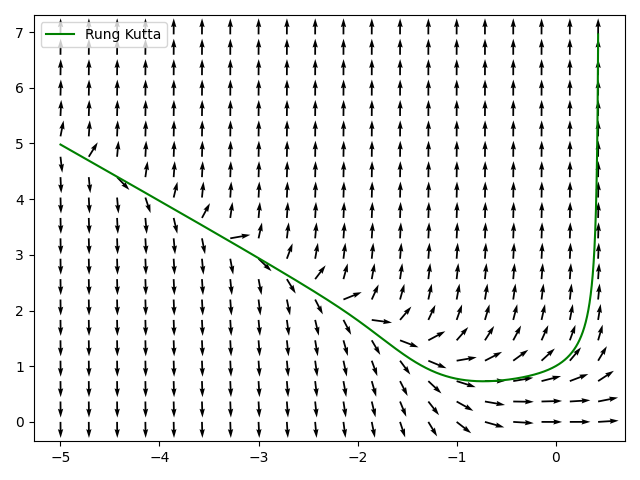
\includegraphics[scale=0.3]{P2FinalSolution.png}
\end{center}

\newpage

\section{Appendix}

\subsection{The Code We Wrote}

This section reveals the code we wrote (in python). We used Github to record our progress and you can also clone and view them with your own IDE. Here is our project's link:

\begin{center}
	\url{https://github.com/QuokeCola/MATH286Lab}
\end{center}

\subsubsection{Euler}\label{Euler}
\scriptsize

\fontspec [ Path = ttf/, 
			UprightFont = *-Medium,
 			BoldFont = *-bold,]
			{JetbrainsMono}

\begin{lstlisting}
	import numpy as np
	class Euler(object):
		point_hist = []
		res = ([],False)
		def __init__(self, diff_func, step, start_point, stop_range):
			self.diff_func = diff_func
			self.step = step
			self.start_point = start_point
			self.stop_range = stop_range
			self.overFlow = False
			self.x = np.arange(start_point[0],stop_range,step)
			self.y = [start_point[1]]
	
		def compute(self):
			print("Start Computing Euler Results")
			end_Str = '100%'
			count = 0
			for i in self.x:
				try:
					f = self.diff_func(i,self.y[len(self.y)-1])
					y_new = self.y[len(self.y)-1]+self.step*f
					self.y.append(y_new)
				except ValueError:
					return [self.x, self.y]
			self.y.pop()
			print("Compute Euler Results Finished")
			return [self.x, self.y]
		
\end{lstlisting}
\subsubsection{Improved Euler(Heun)}\label{Heun}
\begin{lstlisting}
	import numpy as np

	class OptEu(object):
		point_hist = []

		def __init__(self, diff_func, step, start_point, stop_range):
			self.diff_func = diff_func
			self.step = step
			self.start_point = start_point
			self.stop_range = stop_range
			self.overFlow = False
			self.x = np.arange(start_point[0],stop_range,step)
			self.y = [start_point[1]]

		def compute(self):
			print("Start Computing Euler Results")
			count = 0
			for i in self.x:
				try:
					f_low = self.diff_func(i, self.y[len(self.y)-1])
					x_high = i + self.step
					y_high = self.y[len(self.y)-1] + self.step * f_low
					f_high = self.diff_func(x_high, y_high)
					y_new = self.y[len(self.y)-1] + self.step * 0.5 * (f_low + f_high)
					self.y.append(y_new)
				except OverflowError:
					return [self.x, self.y]
			self.y.pop()
			print("Compute Improved Euler Results Finished")
			return [self.x, self.y]
\end{lstlisting}
\subsubsection{Runge Kutta}\label{Runge Kutta}

\begin{lstlisting}
	import numpy as np
	class RunKu(object):
		point_hist = []

		def __init__(self, diff_func, step, start_point, stop_range):
			self.diff_func = diff_func
			self.step = step
			self.start_point = start_point
			self.stop_range = stop_range
			self.overFlow = False
			self.x = np.arange(start_point[0],stop_range,step)
			self.y = [start_point[1]]

		def compute(self):
			print("Start Computing Runge Kutta Results")
			for i in self.x:
				try:
					k1 = self.diff_func(i, self.y[len(self.y)-1])
					x_1 = i + self.step * 0.5
					y_1 = self.y[len(self.y)-1] + self.step * k1 * 0.5
					k2 = self.diff_func(x_1, y_1)
					x_2 = i + self.step * 0.5
					y_2 = self.y[len(self.y)-1] + self.step * k2 * 0.5
					k3 = self.diff_func(x_2, y_2)
					x_3 = i + self.step
					y_3 = self.y[len(self.y)-1] + self.step * k3
					k4 = self.diff_func(x_3, y_3)
					y_new = self.y[len(self.y)-1] + self.step / 6 * (k1 + 2 * (k2 + k3) + k4)
					self.y.append(y_new)
				except OverflowError:
					return [self.x, self.y]
			self.y.pop()
			print("Compute Runge Kutta Results Finished")
			return [self.x, self.y]
\end{lstlisting}

\subsubsection{Analytical Algorithm in Problem 1}

\begin{lstlisting}
	import numpy as np
	import multiprocessing
	class analytical:
		def __init__(self):

			self.a = [0,0,0,0]
			self.a[0] = 1.0
			self.a[1] = self.a[0] ** 2
			self.a[2] = 0.5 * (2 * self.a[0] * self.a[1] + self.a[0])
			self.a[3] = (1 + self.a[1] ** 2 + 2 * self.a[0] * self.a[2] + self.a[1])/3
			self.y_list = []
			self.point_nums = 1

		# @params subs the terms needs to generate. (Number of a n)
		def generate_subs(self, subs):
			print("Start Computing Analytical Subjects")
			while len(self.a) < subs:
				new_a = self.a[len(self.a)-2]
				for i in range(0, len(self.a)):
					new_a += self.a[i]*self.a[len(self.a)-1-i]
				self.a.append(new_a/len(self.a))

			print("Successfully Compute Analytical Subjects")

		def callbackfunc(self, retval):
			self.y_list.append(retval)

		def single_step(self, x):
			y = 0
			y+=self.a[0]
			for i in range(1, len(self.a)):
				y += self.a[i] * (x ** i)
			return y

		# @params end_scale means the t to stop
		# @params point_nums the number of y need to calculated.
		def compute(self, end_scale, point_nums = 2):
			print("Start Compute Analytical Result")
			pool = multiprocessing.Pool()
			x_list = np.linspace(0, end_scale, point_nums)
			self.point_nums = point_nums

			for item in x_list:
				# Using multiple Cores to decrease the calculate time.
				pool.apply_async(self.single_step,[item],callback=self.callbackfunc) 
			pool.close()
			pool.join()
			print("Successfully Compute Analytical Result")
			return (x_list, self.y_list)
\end{lstlisting}

\subsubsection{Main File}
\begin{lstlisting}
	from __future__ import division
	import sys

	import warnings
	warnings.filterwarnings("ignore")

	from Euler_Method import *
	from Opt_Euler_Method import *
	from RungKutta_Method import *
	from analytical import *
	from Function_DF import *

	import matplotlib.pyplot as plt
	import numpy as np
	import time
	sys.setrecursionlimit(100000)

	start_Point = (0, 1)
	Step = 0.0000001
	HigherScale = 0.43
	LowerScale = -5

	Prob1AnalyticalEnable = False
	GraphicEnable = True

	Analytical_Subjects = 1000
	Analytical_Points = 100
	enable_safe_print = False


	def diffF(x,y):
		return y*y+x*y+x*x

	def Single_Calculation(Step, end_Scale):

		euler = Euler(diffF, Step, start_Point, end_Scale)
		optEu = OptEu(diffF, Step, start_Point, end_Scale)
		runKu = RunKu(diffF, Step, start_Point, end_Scale)
		start_time = time.time()
		EulRes = euler.compute()
		end_time = time.time()
		print("Euler Algorithm Spent Time:" + str(end_time - start_time) + 'seconds')
		start_time = time.time()
		OptEuRes = optEu.compute()
		end_time = time.time()
		print("Improved Euler Algorithm Spent Time:" + str(end_time - start_time) + 'seconds')
		start_time = time.time()
		RunKuRes = runKu.compute()
		end_time = time.time()
		print("Runge Kutta Algorithm Spent Time:" + str(end_time - start_time) + 'seconds')
		return (EulRes, OptEuRes, RunKuRes, end_Scale)

	def showRes(ResTup):
		print('-----------------Trial '+str(ResTup[3]) +'-----------------')
		if not (str(ResTup[0][1][-1]).find('inf') == -1) and enable_safe_print:
			print('Euler Overflow')
		else:
			print('Euler: ' + str(ResTup[0][1][-1]))

		if not (str(ResTup[1][1][-1]).find('inf') == -1) and enable_safe_print:
			print('Advanced Euler Overflow')
		else:
			print('Opt Euler: ' + str(ResTup[1][1][-1]))
		if not (str(ResTup[2][1][-1]).find('inf') == -1) and enable_safe_print:
			print('Rung Kutta Overflow')
		else:
			print('Rung Kutta: ' + str(ResTup[2][1][-1]))

	def log_Res(Res):
		file = open('result.csv','w')
		header = 'x,Euler, Advanced Euler, Rung Kutta\n'
		lines = [header]
		for i in range(len(Res[0][0])):
			lines.append(str(Res[2][0][i])+','+ str(Res[0][1][i])+ ',' + str(Res[1][1][i])+ ','+str(Res[2][1][i])+ '\n')
		file.writelines(lines)
		file.close()

	if __name__ == '__main__':

		# Run Calculation
		print("Start Computing Numerical Results")
		PosRes=Single_Calculation(Step, HigherScale)
		NegRes=Single_Calculation(-Step, LowerScale)
		Res = [[np.hstack((NegRes[0][0][::-1], PosRes[0][0])), np.hstack((NegRes[0][1][::-1], PosRes[0][1]))],
			  [np.hstack((NegRes[1][0][::-1], PosRes[1][0])), np.hstack((NegRes[1][1][::-1], PosRes[1][1]))],
			  [np.hstack((NegRes[2][0][::-1], PosRes[2][0])), np.hstack((NegRes[2][1][::-1], PosRes[2][1]))]]

		print("Numerical Compute Finished")
		showRes(Res)
		print('Start log Results')
		log_Res(Res)
		print('Log Results Finished')

		# Run Analytical Results
		if (Prob1AnalyticalEnable):
			analy = analytical()
			analy.generate_subs(Analytical_Subjects)
			anares = analy.compute(HigherScale, Analytical_Points)

		# Plot Direction Field
		LowX = NegRes[0][0][-1]
		HighX = PosRes[0][0][-1]
		LowY = NegRes[2][1][-1]
		HighY = start_Point[1]
		for i in range(len(PosRes[2][1])):
			if not str(PosRes[2][1][i]).find('inf') == -1:
				HighY = PosRes[2][1][i - 1]
				print(HighY)
				break
		if Prob1AnalyticalEnable:
			for i in range(len(anares[1])):
				if not str(anares[1][i]).find('inf') == -1:
					HighY = anares[1][i-1]
					print(HighY)
					break
			if HighY == start_Point[1]:
				HighY = anares[1][-1]
		HighY = PosRes[2][1][-1]
		if GraphicEnable:
			funcDF = FunDF(diffF,LowX,HighX,0,HighY,20,20)
			funcDF.generate()

			# Plot Points
			print("Add points to plot")
			plt.plot(Res[0][0], Res[0][1], '-', color ='blue', label ='Euler')
			plt.plot(Res[1][0], Res[1][1], '-', color ='red', label ='OptEuler')
			plt.plot(Res[2][0], Res[2][1], '-', color ='green', label ='Rung Kutta')
			if Prob1AnalyticalEnable:
				plt.plot(anares[0], anares[1], color = 'purple', label ='Analysis')
			plt.legend(loc = 'best')
			print("Points added to plot")
			print("Generating plot")
			plt.show()
			print("Plot Generated")
\end{lstlisting}
\end{document}